% Health Campaigns
% Compile with: latexmk -pdf health_campaigns.tex
\documentclass[aspectratio=169,11pt]{beamer}

\usepackage[T1]{fontenc}
\usepackage{lmodern}
\usepackage{booktabs}
\usepackage{array}
\usepackage{tikz}
\usetikzlibrary{shapes.geometric,positioning,calc,arrows.meta}
\usepackage{pgfplots}
\pgfplotsset{compat=1.18}
\usepackage[most]{tcolorbox}
\graphicspath{{images/}}

% ---------- Colors ----------
\definecolor{navy}{HTML}{1C2541}
\definecolor{oldred}{HTML}{B22234}   % US flag red, also the accent color
\definecolor{oldblue}{HTML}{3C3B6E}  % US flag blue
\definecolor{ink}{HTML}{2B2B2B}
\definecolor{muted}{HTML}{8A8F98}
\definecolor{paper}{HTML}{FFFFFF}
\definecolor{dem}{HTML}{2E5FA3}      % Democrats
\definecolor{rep}{HTML}{C0392B}      % Republicans
\definecolor{austria}{HTML}{C8102E}  % Austria red, for USA-vs-Austria comparisons

% ---------- Minimal theme ----------
\setbeamertemplate{navigation symbols}{}
\setbeamercolor{normal text}{fg=ink, bg=paper}
\setbeamercolor{structure}{fg=navy}
\setbeamercolor{frametitle}{fg=navy}
\setbeamercolor{alerted text}{fg=oldred}
\setbeamercolor{footnote}{fg=muted}
\setbeamerfont{frametitle}{size=\Large, series=\bfseries}
\setbeamertemplate{itemize item}{\color{oldred}\textbullet}
\setbeamertemplate{itemize subitem}{\color{muted}--}
\setbeamertemplate{enumerate item}{\color{oldred}\insertenumlabel.}
\setbeamersize{text margin left=1.1cm, text margin right=1.1cm}
\hypersetup{colorlinks=true, urlcolor=dem, linkcolor=navy}

\setbeamertemplate{frametitle}{%
  \vspace*{0.5cm}%
  \usebeamerfont{frametitle}\usebeamercolor[fg]{frametitle}\insertframetitle\par
  \vspace{0.15cm}{\color{navy!15}\rule{\textwidth}{0.4pt}}\par}

\setbeamertemplate{footline}{%
  \hfill{\tiny\color{muted}\insertframenumber}\hspace*{0.6cm}\vspace*{0.35cm}}

% Plain divider at the start of each section
\AtBeginSection{%
  \begin{frame}[plain,noframenumbering]
    \centering
    {\LARGE\bfseries\color{navy}\insertsection}\\[0.6em]
    {\color{oldred}\rule{1.5cm}{0.8pt}}
  \end{frame}}

% "Think" question slides: \begin{thinkframe} ... \end{thinkframe}
\newenvironment{thinkframe}{%
  \begin{frame}[plain,noframenumbering,environment=thinkframe]\centering\Large}{\end{frame}}

% ---------- Helpers ----------
% Small grey source line at the bottom of a frame
\newcommand{\source}[1]{%
  \begin{tikzpicture}[remember picture,overlay]
    \node[anchor=south west, font=\tiny, text=muted, text width=0.85\paperwidth, align=left]
      at ($(current page.south west)+(0.6cm,0.25cm)$) {#1};
  \end{tikzpicture}}

% Quote box with a thin red rule on the left; optional arg e.g. [fontupper=\itshape\small]
\newtcolorbox{textquote}[1][]{%
  enhanced, frame hidden, boxrule=0pt, sharp corners,
  colback=navy!4, borderline west={2pt}{0pt}{oldred},
  left=10pt, right=8pt, top=6pt, bottom=6pt, fontupper=\itshape, #1}

% Photo + name + short bio (use inside a column): \candidate{file}{Name}{bio}
\newcommand{\candidate}[3]{%
  \begin{minipage}[t]{\linewidth}\centering
    \includegraphics[height=3.5cm]{#1}\\[0.5em]
    {\large\bfseries\color{navy}#2}\\[0.4em]
    \begin{minipage}{0.9\linewidth}\raggedright\small #3\end{minipage}
  \end{minipage}}

% Big number with a caption (use inside a column): \bignum{color}{91\%}{caption}
\newcommand{\bignum}[3]{%
  \begin{minipage}[t]{\linewidth}\centering
    {\fontsize{34}{38}\selectfont\bfseries\color{#1}#2}\\[0.3em]
    {\small #3}
  \end{minipage}}

% US flag drawn in TikZ (hoist height = #1), e.g. \usflag{3cm}
\newcommand{\usflag}[1]{%
  \begin{tikzpicture}[x=#1, y=#1]
    \def\fly{1.9}
    \foreach \i in {0,...,12} {
      \pgfmathsetmacro{\c}{mod(\i,2)==0 ? 1 : 0}
      \ifdim\c pt=1pt
        \fill[oldred] (0,{1-(\i+1)/13}) rectangle (\fly,{1-\i/13});
      \else
        \fill[white] (0,{1-(\i+1)/13}) rectangle (\fly,{1-\i/13});
      \fi
    }
    \def\cw{0.76} \def\ch{0.5385}
    \fill[oldblue] (0,{1-\ch}) rectangle (\cw,1);
    \foreach \r in {1,...,9} {
      \pgfmathsetmacro{\isodd}{mod(\r,2)}
      \ifdim\isodd pt=1pt
        \foreach \k in {0,...,5}
          \node[star, star points=5, star point ratio=2.618, fill=white, inner sep=0pt,
                minimum size=0.0616*#1] at ({(2*\k+1)*\cw/12},{1-\r*\ch/10}) {};
      \else
        \foreach \k in {0,...,4}
          \node[star, star points=5, star point ratio=2.618, fill=white, inner sep=0pt,
                minimum size=0.0616*#1] at ({(2*\k+2)*\cw/12},{1-\r*\ch/10}) {};
      \fi
    }
    \draw[ink!30, line width=0.3pt] (0,0) rectangle (\fly,1);
  \end{tikzpicture}}

% Agree/disagree spectrum for "spectrum game" activities
\newcommand{\spectrum}{%
  
\begin{tikzpicture}
    \shade[left color=oldblue, right color=oldred, rounded corners=2pt] (0,0) rectangle (11,0.18);
    \node[anchor=north, font=\small, text=oldblue] at (0,-0.15) {Strongly disagree};
    \node[anchor=north, font=\small, text=muted] at (5.5,-0.15) {Neutral};
    \node[anchor=north, font=\small, text=oldred] at (11,-0.15) {Strongly agree};
    \fill[paper, draw=muted] (5.5,0.09) circle (2.5pt);
  \end{tikzpicture}}

% One statement per slide: \statement{number}{total}{text}
\newcommand{\statement}[3]{%
  \begin{frame}[plain]
    \vfill
    \begin{center}
      {\small\color{muted}Statement #1 of #2}\\[1.2em]
      {\LARGE\bfseries #3}
    \end{center}
    \vfill
    \begin{center}\spectrum\end{center}
    \vspace{1.2cm}
  \end{frame}}

\begin{document}

\begin{frame}[plain]
  \centering
  {\fontsize{34}{40}\selectfont\bfseries\color{navy} Health Campaigns}\\[0.8em]
  {\color{oldred}\rule{3cm}{1.5pt}}
\end{frame}

\begin{frame}[plain]
  \centering{\LARGE\bfseries\color{navy} How long is a healthy life?}
\end{frame}
\begin{frame}{How long is a healthy life?}
  \begin{itemize}\setlength{\itemsep}{0.9em}
    \item Average U.S. lifespan: \alert{79 years}
    \item E.U. lifespan: \alert{81.5 years}
    \item Monaco has the world's highest life expectancy: \alert{86.7 years}
  \end{itemize}
  \source{Sources: CDC (2024); Eurostat (2024); Worldometer, from UN estimates (Monaco).}
\end{frame}
\begin{frame}[plain]
  \begin{columns}[c]
    \begin{column}{0.52\textwidth}\centering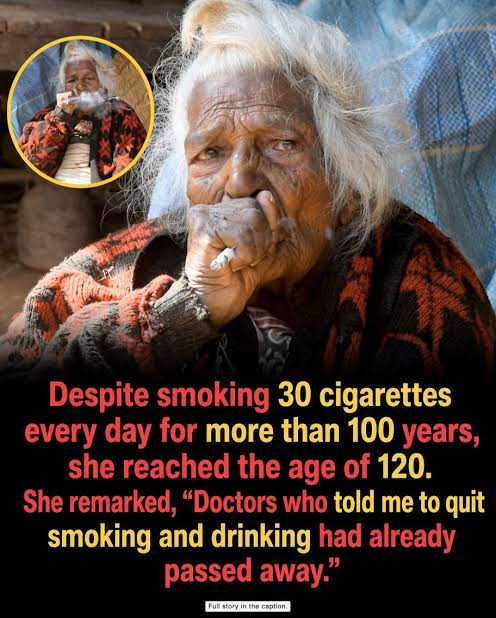
\includegraphics[height=8cm]{old_smoker.jpg}\end{column}
    \begin{column}{0.42\textwidth}
      \begin{itemize}\item {\large Genetic variation can complicate this}\end{itemize}
    \end{column}
  \end{columns}
\end{frame}
\begin{frame}{America's biggest health concerns}
  \relax{\small\color{muted}Leading causes of death (according to the CDC)\par}\vspace{-0.2em}
  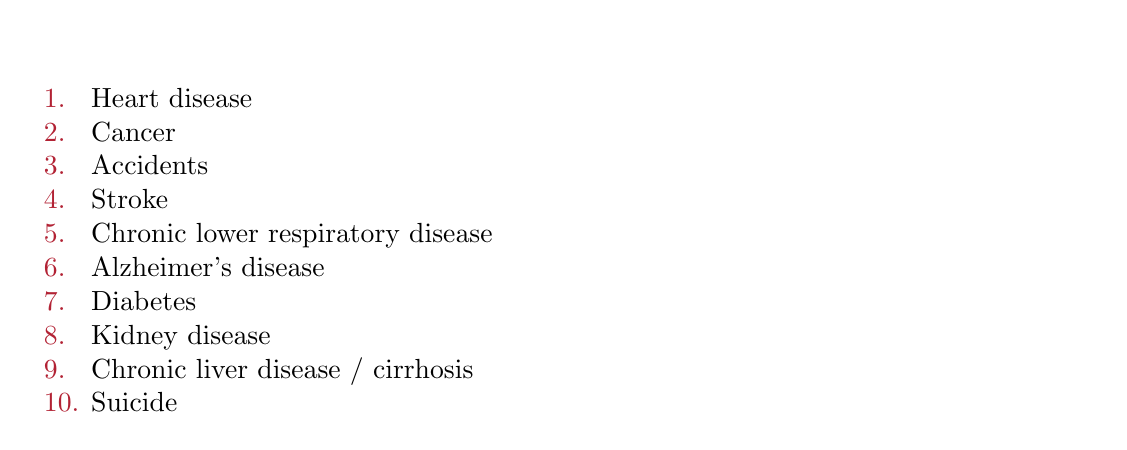
\begin{tikzpicture}[x=1cm,y=-0.43cm]
    \path (0,-1.35) rectangle (13.6,10.3);
    \node[anchor=base west,inner sep=0] at (0.2,1) {\makebox[0.6cm][l]{\color{oldred}1.}Heart disease};
    \node[anchor=base west,inner sep=0] at (0.2,2) {\makebox[0.6cm][l]{\color{oldred}2.}Cancer};
    \node[anchor=base west,inner sep=0] at (0.2,3) {\makebox[0.6cm][l]{\color{oldred}3.}Accidents};
    \node[anchor=base west,inner sep=0] at (0.2,4) {\makebox[0.6cm][l]{\color{oldred}4.}Stroke};
    \node[anchor=base west,inner sep=0] at (0.2,5) {\makebox[0.6cm][l]{\color{oldred}5.}Chronic lower respiratory disease};
    \node[anchor=base west,inner sep=0] at (0.2,6) {\makebox[0.6cm][l]{\color{oldred}6.}Alzheimer's disease};
    \node[anchor=base west,inner sep=0] at (0.2,7) {\makebox[0.6cm][l]{\color{oldred}7.}Diabetes};
    \node[anchor=base west,inner sep=0] at (0.2,8) {\makebox[0.6cm][l]{\color{oldred}8.}Kidney disease};
    \node[anchor=base west,inner sep=0] at (0.2,9) {\makebox[0.6cm][l]{\color{oldred}9.}Chronic liver disease / cirrhosis};
    \node[anchor=base west,inner sep=0] at (0.2,10) {\makebox[0.6cm][l]{\color{oldred}10.}Suicide};
  \end{tikzpicture}
  \source{Causes of death: CDC, final data for 2024.}
\end{frame}
\begin{frame}{America's biggest health concerns \mdseries + lack of sleep}
  \relax{\small\color{muted}Leading causes of death (according to the CDC)\par}\vspace{-0.2em}
  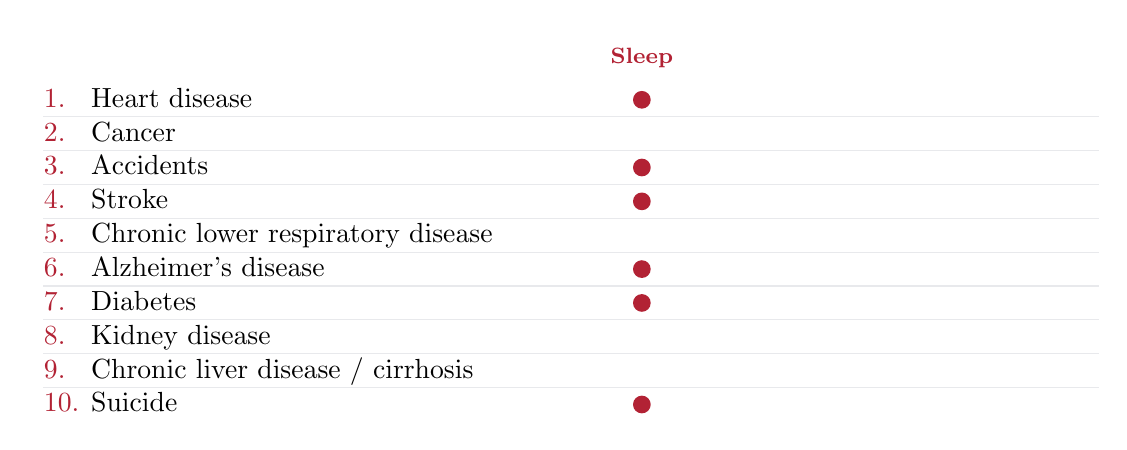
\begin{tikzpicture}[x=1cm,y=-0.43cm]
    \path (0,-1.35) rectangle (13.6,10.3);
    \node[anchor=base west,inner sep=0] at (0.2,1) {\makebox[0.6cm][l]{\color{oldred}1.}Heart disease};
    \node[anchor=base west,inner sep=0] at (0.2,2) {\makebox[0.6cm][l]{\color{oldred}2.}Cancer};
    \node[anchor=base west,inner sep=0] at (0.2,3) {\makebox[0.6cm][l]{\color{oldred}3.}Accidents};
    \node[anchor=base west,inner sep=0] at (0.2,4) {\makebox[0.6cm][l]{\color{oldred}4.}Stroke};
    \node[anchor=base west,inner sep=0] at (0.2,5) {\makebox[0.6cm][l]{\color{oldred}5.}Chronic lower respiratory disease};
    \node[anchor=base west,inner sep=0] at (0.2,6) {\makebox[0.6cm][l]{\color{oldred}6.}Alzheimer's disease};
    \node[anchor=base west,inner sep=0] at (0.2,7) {\makebox[0.6cm][l]{\color{oldred}7.}Diabetes};
    \node[anchor=base west,inner sep=0] at (0.2,8) {\makebox[0.6cm][l]{\color{oldred}8.}Kidney disease};
    \node[anchor=base west,inner sep=0] at (0.2,9) {\makebox[0.6cm][l]{\color{oldred}9.}Chronic liver disease / cirrhosis};
    \node[anchor=base west,inner sep=0] at (0.2,10) {\makebox[0.6cm][l]{\color{oldred}10.}Suicide};
    \node[anchor=center,align=center,font=\footnotesize\bfseries,text=oldred] at (7.8,-0.45) {Sleep};
    \fill[oldred] (7.8,0.78) circle (3.2pt);
    \fill[oldred] (7.8,2.78) circle (3.2pt);
    \fill[oldred] (7.8,3.78) circle (3.2pt);
    \fill[oldred] (7.8,5.78) circle (3.2pt);
    \fill[oldred] (7.8,6.78) circle (3.2pt);
    \fill[oldred] (7.8,9.78) circle (3.2pt);
    \draw[navy!10] (0.2,1.28) -- (13.6,1.28);
    \draw[navy!10] (0.2,2.2800000000000002) -- (13.6,2.2800000000000002);
    \draw[navy!10] (0.2,3.2800000000000002) -- (13.6,3.2800000000000002);
    \draw[navy!10] (0.2,4.28) -- (13.6,4.28);
    \draw[navy!10] (0.2,5.28) -- (13.6,5.28);
    \draw[navy!10] (0.2,6.28) -- (13.6,6.28);
    \draw[navy!10] (0.2,7.28) -- (13.6,7.28);
    \draw[navy!10] (0.2,8.28) -- (13.6,8.28);
    \draw[navy!10] (0.2,9.28) -- (13.6,9.28);
  \end{tikzpicture}
  \source{Causes of death: CDC, final data for 2024.}
\end{frame}
\begin{frame}{America's biggest health concerns \mdseries + unhealthy diet}
  \relax{\small\color{muted}Leading causes of death (according to the CDC)\par}\vspace{-0.2em}
  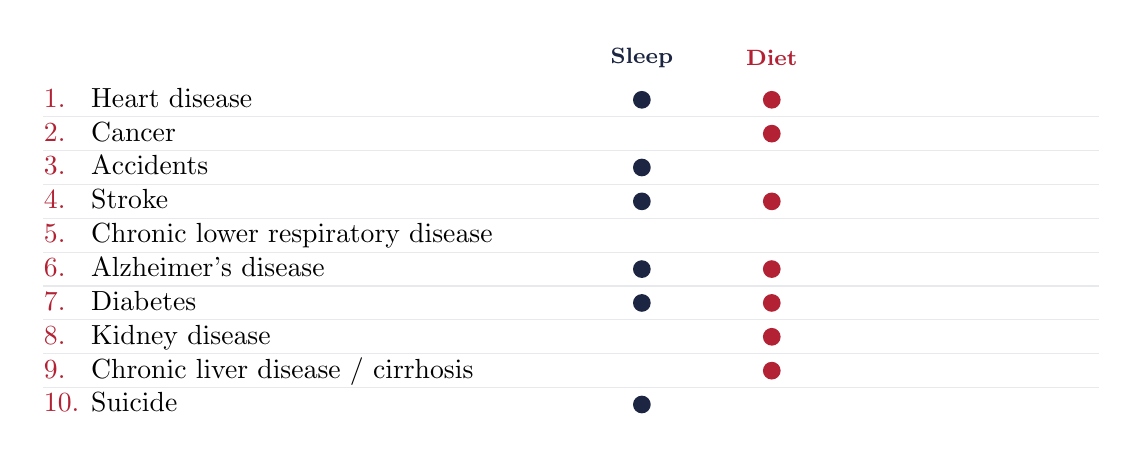
\begin{tikzpicture}[x=1cm,y=-0.43cm]
    \path (0,-1.35) rectangle (13.6,10.3);
    \node[anchor=base west,inner sep=0] at (0.2,1) {\makebox[0.6cm][l]{\color{oldred}1.}Heart disease};
    \node[anchor=base west,inner sep=0] at (0.2,2) {\makebox[0.6cm][l]{\color{oldred}2.}Cancer};
    \node[anchor=base west,inner sep=0] at (0.2,3) {\makebox[0.6cm][l]{\color{oldred}3.}Accidents};
    \node[anchor=base west,inner sep=0] at (0.2,4) {\makebox[0.6cm][l]{\color{oldred}4.}Stroke};
    \node[anchor=base west,inner sep=0] at (0.2,5) {\makebox[0.6cm][l]{\color{oldred}5.}Chronic lower respiratory disease};
    \node[anchor=base west,inner sep=0] at (0.2,6) {\makebox[0.6cm][l]{\color{oldred}6.}Alzheimer's disease};
    \node[anchor=base west,inner sep=0] at (0.2,7) {\makebox[0.6cm][l]{\color{oldred}7.}Diabetes};
    \node[anchor=base west,inner sep=0] at (0.2,8) {\makebox[0.6cm][l]{\color{oldred}8.}Kidney disease};
    \node[anchor=base west,inner sep=0] at (0.2,9) {\makebox[0.6cm][l]{\color{oldred}9.}Chronic liver disease / cirrhosis};
    \node[anchor=base west,inner sep=0] at (0.2,10) {\makebox[0.6cm][l]{\color{oldred}10.}Suicide};
    \node[anchor=center,align=center,font=\footnotesize\bfseries,text=navy] at (7.8,-0.45) {Sleep};
    \fill[navy] (7.8,0.78) circle (3.2pt);
    \fill[navy] (7.8,2.78) circle (3.2pt);
    \fill[navy] (7.8,3.78) circle (3.2pt);
    \fill[navy] (7.8,5.78) circle (3.2pt);
    \fill[navy] (7.8,6.78) circle (3.2pt);
    \fill[navy] (7.8,9.78) circle (3.2pt);
    \node[anchor=center,align=center,font=\footnotesize\bfseries,text=oldred] at (9.45,-0.45) {Diet};
    \fill[oldred] (9.45,0.78) circle (3.2pt);
    \fill[oldred] (9.45,1.78) circle (3.2pt);
    \fill[oldred] (9.45,3.78) circle (3.2pt);
    \fill[oldred] (9.45,5.78) circle (3.2pt);
    \fill[oldred] (9.45,6.78) circle (3.2pt);
    \fill[oldred] (9.45,7.78) circle (3.2pt);
    \fill[oldred] (9.45,8.78) circle (3.2pt);
    \draw[navy!10] (0.2,1.28) -- (13.6,1.28);
    \draw[navy!10] (0.2,2.2800000000000002) -- (13.6,2.2800000000000002);
    \draw[navy!10] (0.2,3.2800000000000002) -- (13.6,3.2800000000000002);
    \draw[navy!10] (0.2,4.28) -- (13.6,4.28);
    \draw[navy!10] (0.2,5.28) -- (13.6,5.28);
    \draw[navy!10] (0.2,6.28) -- (13.6,6.28);
    \draw[navy!10] (0.2,7.28) -- (13.6,7.28);
    \draw[navy!10] (0.2,8.28) -- (13.6,8.28);
    \draw[navy!10] (0.2,9.28) -- (13.6,9.28);
  \end{tikzpicture}
  \source{Causes of death: CDC, final data for 2024.}
\end{frame}
\begin{frame}{America's biggest health concerns \mdseries + infrequent exercise}
  \relax{\small\color{muted}Leading causes of death (according to the CDC)\par}\vspace{-0.2em}
  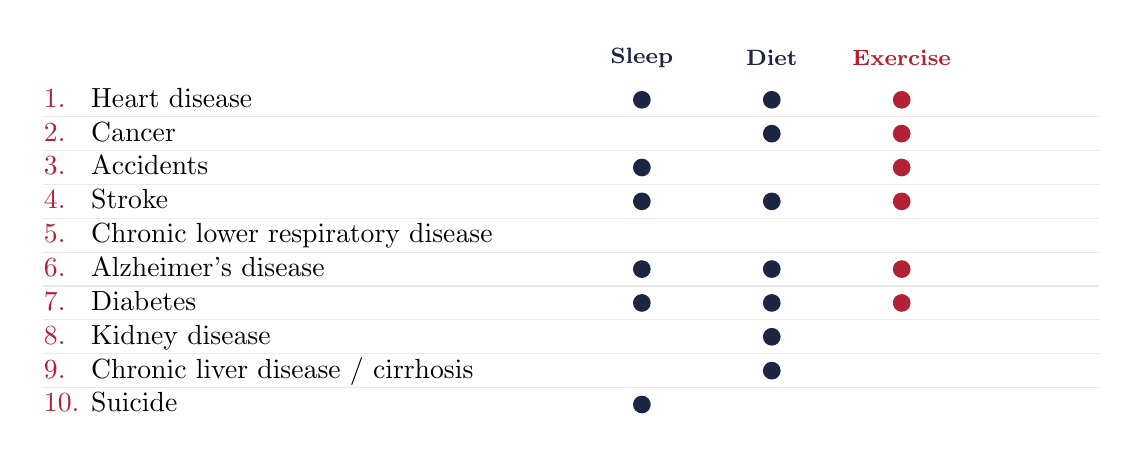
\begin{tikzpicture}[x=1cm,y=-0.43cm]
    \path (0,-1.35) rectangle (13.6,10.3);
    \node[anchor=base west,inner sep=0] at (0.2,1) {\makebox[0.6cm][l]{\color{oldred}1.}Heart disease};
    \node[anchor=base west,inner sep=0] at (0.2,2) {\makebox[0.6cm][l]{\color{oldred}2.}Cancer};
    \node[anchor=base west,inner sep=0] at (0.2,3) {\makebox[0.6cm][l]{\color{oldred}3.}Accidents};
    \node[anchor=base west,inner sep=0] at (0.2,4) {\makebox[0.6cm][l]{\color{oldred}4.}Stroke};
    \node[anchor=base west,inner sep=0] at (0.2,5) {\makebox[0.6cm][l]{\color{oldred}5.}Chronic lower respiratory disease};
    \node[anchor=base west,inner sep=0] at (0.2,6) {\makebox[0.6cm][l]{\color{oldred}6.}Alzheimer's disease};
    \node[anchor=base west,inner sep=0] at (0.2,7) {\makebox[0.6cm][l]{\color{oldred}7.}Diabetes};
    \node[anchor=base west,inner sep=0] at (0.2,8) {\makebox[0.6cm][l]{\color{oldred}8.}Kidney disease};
    \node[anchor=base west,inner sep=0] at (0.2,9) {\makebox[0.6cm][l]{\color{oldred}9.}Chronic liver disease / cirrhosis};
    \node[anchor=base west,inner sep=0] at (0.2,10) {\makebox[0.6cm][l]{\color{oldred}10.}Suicide};
    \node[anchor=center,align=center,font=\footnotesize\bfseries,text=navy] at (7.8,-0.45) {Sleep};
    \fill[navy] (7.8,0.78) circle (3.2pt);
    \fill[navy] (7.8,2.78) circle (3.2pt);
    \fill[navy] (7.8,3.78) circle (3.2pt);
    \fill[navy] (7.8,5.78) circle (3.2pt);
    \fill[navy] (7.8,6.78) circle (3.2pt);
    \fill[navy] (7.8,9.78) circle (3.2pt);
    \node[anchor=center,align=center,font=\footnotesize\bfseries,text=navy] at (9.45,-0.45) {Diet};
    \fill[navy] (9.45,0.78) circle (3.2pt);
    \fill[navy] (9.45,1.78) circle (3.2pt);
    \fill[navy] (9.45,3.78) circle (3.2pt);
    \fill[navy] (9.45,5.78) circle (3.2pt);
    \fill[navy] (9.45,6.78) circle (3.2pt);
    \fill[navy] (9.45,7.78) circle (3.2pt);
    \fill[navy] (9.45,8.78) circle (3.2pt);
    \node[anchor=center,align=center,font=\footnotesize\bfseries,text=oldred] at (11.1,-0.45) {Exercise};
    \fill[oldred] (11.1,0.78) circle (3.2pt);
    \fill[oldred] (11.1,1.78) circle (3.2pt);
    \fill[oldred] (11.1,2.78) circle (3.2pt);
    \fill[oldred] (11.1,3.78) circle (3.2pt);
    \fill[oldred] (11.1,5.78) circle (3.2pt);
    \fill[oldred] (11.1,6.78) circle (3.2pt);
    \draw[navy!10] (0.2,1.28) -- (13.6,1.28);
    \draw[navy!10] (0.2,2.2800000000000002) -- (13.6,2.2800000000000002);
    \draw[navy!10] (0.2,3.2800000000000002) -- (13.6,3.2800000000000002);
    \draw[navy!10] (0.2,4.28) -- (13.6,4.28);
    \draw[navy!10] (0.2,5.28) -- (13.6,5.28);
    \draw[navy!10] (0.2,6.28) -- (13.6,6.28);
    \draw[navy!10] (0.2,7.28) -- (13.6,7.28);
    \draw[navy!10] (0.2,8.28) -- (13.6,8.28);
    \draw[navy!10] (0.2,9.28) -- (13.6,9.28);
  \end{tikzpicture}
  \source{Causes of death: CDC, final data for 2024.}
\end{frame}
\begin{frame}{America's biggest health concerns \mdseries + smoking or drinking}
  \relax{\small\color{muted}Leading causes of death (according to the CDC)\par}\vspace{-0.2em}
  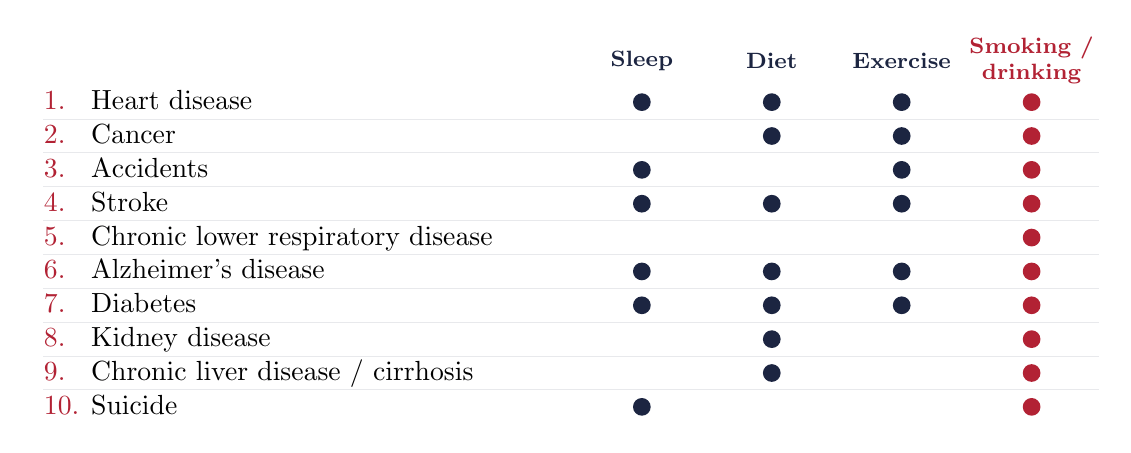
\begin{tikzpicture}[x=1cm,y=-0.43cm]
    \path (0,-1.35) rectangle (13.6,10.3);
    \node[anchor=base west,inner sep=0] at (0.2,1) {\makebox[0.6cm][l]{\color{oldred}1.}Heart disease};
    \node[anchor=base west,inner sep=0] at (0.2,2) {\makebox[0.6cm][l]{\color{oldred}2.}Cancer};
    \node[anchor=base west,inner sep=0] at (0.2,3) {\makebox[0.6cm][l]{\color{oldred}3.}Accidents};
    \node[anchor=base west,inner sep=0] at (0.2,4) {\makebox[0.6cm][l]{\color{oldred}4.}Stroke};
    \node[anchor=base west,inner sep=0] at (0.2,5) {\makebox[0.6cm][l]{\color{oldred}5.}Chronic lower respiratory disease};
    \node[anchor=base west,inner sep=0] at (0.2,6) {\makebox[0.6cm][l]{\color{oldred}6.}Alzheimer's disease};
    \node[anchor=base west,inner sep=0] at (0.2,7) {\makebox[0.6cm][l]{\color{oldred}7.}Diabetes};
    \node[anchor=base west,inner sep=0] at (0.2,8) {\makebox[0.6cm][l]{\color{oldred}8.}Kidney disease};
    \node[anchor=base west,inner sep=0] at (0.2,9) {\makebox[0.6cm][l]{\color{oldred}9.}Chronic liver disease / cirrhosis};
    \node[anchor=base west,inner sep=0] at (0.2,10) {\makebox[0.6cm][l]{\color{oldred}10.}Suicide};
    \node[anchor=center,align=center,font=\footnotesize\bfseries,text=navy] at (7.8,-0.45) {Sleep};
    \fill[navy] (7.8,0.78) circle (3.2pt);
    \fill[navy] (7.8,2.78) circle (3.2pt);
    \fill[navy] (7.8,3.78) circle (3.2pt);
    \fill[navy] (7.8,5.78) circle (3.2pt);
    \fill[navy] (7.8,6.78) circle (3.2pt);
    \fill[navy] (7.8,9.78) circle (3.2pt);
    \node[anchor=center,align=center,font=\footnotesize\bfseries,text=navy] at (9.45,-0.45) {Diet};
    \fill[navy] (9.45,0.78) circle (3.2pt);
    \fill[navy] (9.45,1.78) circle (3.2pt);
    \fill[navy] (9.45,3.78) circle (3.2pt);
    \fill[navy] (9.45,5.78) circle (3.2pt);
    \fill[navy] (9.45,6.78) circle (3.2pt);
    \fill[navy] (9.45,7.78) circle (3.2pt);
    \fill[navy] (9.45,8.78) circle (3.2pt);
    \node[anchor=center,align=center,font=\footnotesize\bfseries,text=navy] at (11.1,-0.45) {Exercise};
    \fill[navy] (11.1,0.78) circle (3.2pt);
    \fill[navy] (11.1,1.78) circle (3.2pt);
    \fill[navy] (11.1,2.78) circle (3.2pt);
    \fill[navy] (11.1,3.78) circle (3.2pt);
    \fill[navy] (11.1,5.78) circle (3.2pt);
    \fill[navy] (11.1,6.78) circle (3.2pt);
    \node[anchor=center,align=center,font=\footnotesize\bfseries,text=oldred] at (12.75,-0.45) {Smoking /\\drinking};
    \fill[oldred] (12.75,0.78) circle (3.2pt);
    \fill[oldred] (12.75,1.78) circle (3.2pt);
    \fill[oldred] (12.75,2.78) circle (3.2pt);
    \fill[oldred] (12.75,3.78) circle (3.2pt);
    \fill[oldred] (12.75,4.78) circle (3.2pt);
    \fill[oldred] (12.75,5.78) circle (3.2pt);
    \fill[oldred] (12.75,6.78) circle (3.2pt);
    \fill[oldred] (12.75,7.78) circle (3.2pt);
    \fill[oldred] (12.75,8.78) circle (3.2pt);
    \fill[oldred] (12.75,9.78) circle (3.2pt);
    \draw[navy!10] (0.2,1.28) -- (13.6,1.28);
    \draw[navy!10] (0.2,2.2800000000000002) -- (13.6,2.2800000000000002);
    \draw[navy!10] (0.2,3.2800000000000002) -- (13.6,3.2800000000000002);
    \draw[navy!10] (0.2,4.28) -- (13.6,4.28);
    \draw[navy!10] (0.2,5.28) -- (13.6,5.28);
    \draw[navy!10] (0.2,6.28) -- (13.6,6.28);
    \draw[navy!10] (0.2,7.28) -- (13.6,7.28);
    \draw[navy!10] (0.2,8.28) -- (13.6,8.28);
    \draw[navy!10] (0.2,9.28) -- (13.6,9.28);
  \end{tikzpicture}
  \source{Causes of death: CDC, final data for 2024.}
\end{frame}
\begin{frame}{What does a healthy life look like?}
  \begin{itemize}\setlength{\itemsep}{0.9em}
    \item Balanced diet
    \item Frequent exercise
    \item Regular sleep
    \item Not smoking or drinking
  \end{itemize}
\end{frame}
\begin{frame}{How can we promote this? \mdseries Balanced diet: food pyramids}
  \centering
  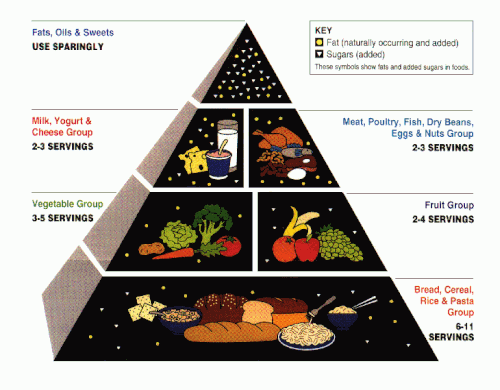
\includegraphics[height=5.9cm,width=\textwidth,keepaspectratio]{pyramid_1992.png}
  \source{Food Guide Pyramid, 1992. Image: USDA, public domain.}
\end{frame}
\begin{frame}{How can we promote this? \mdseries Balanced diet: food pyramids}
  \centering
  
\includegraphics[height=5.9cm,width=\textwidth,keepaspectratio]{myplate.png}
  \source{MyPlate, 2011. Image: USDA, public domain.}
\end{frame}
\begin{frame}{How can we promote this? \mdseries Balanced diet: food pyramids}
  \centering
  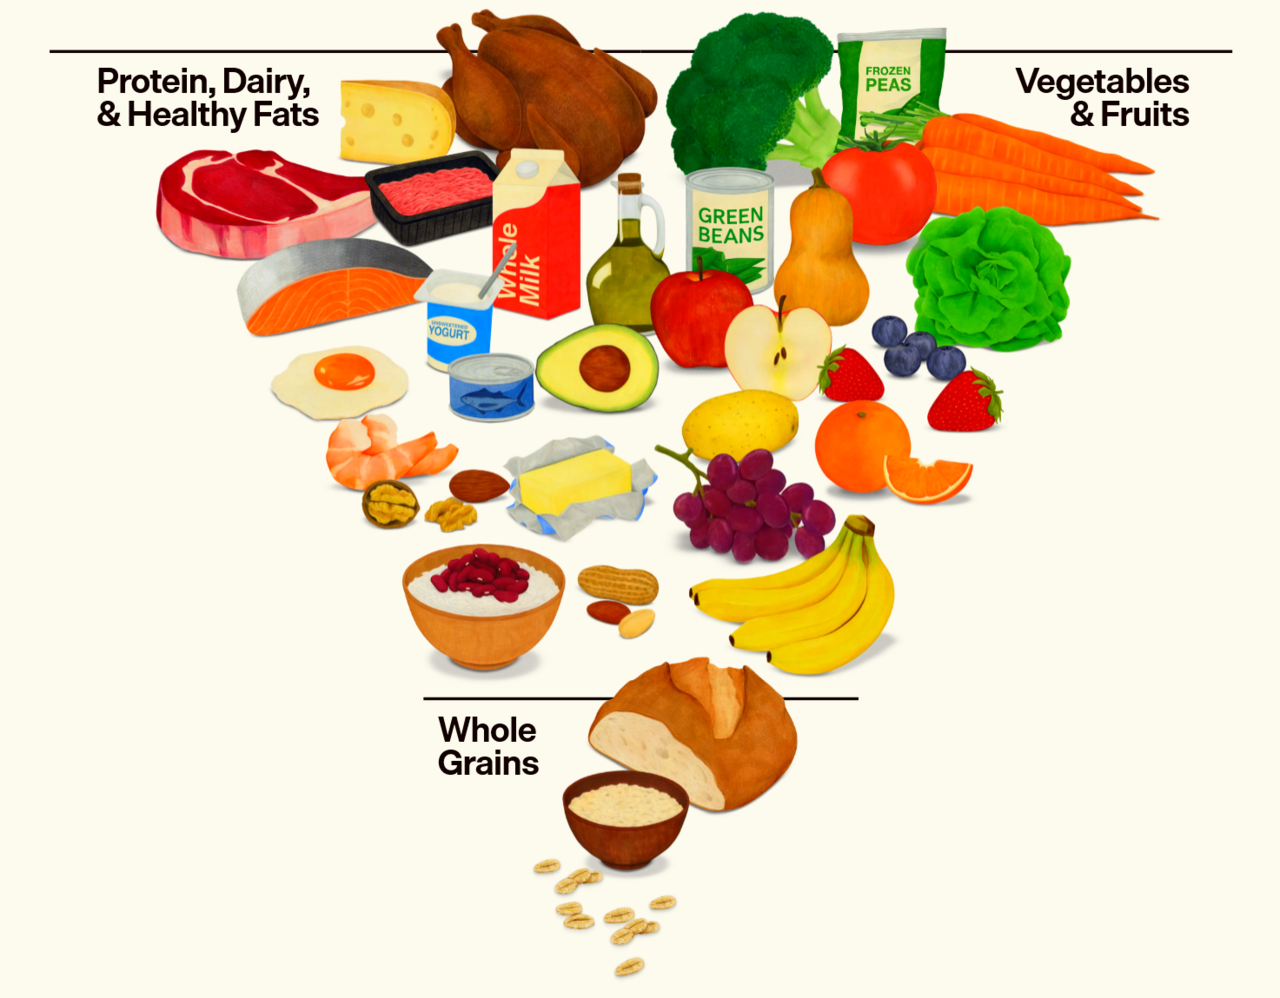
\includegraphics[height=5.9cm,width=\textwidth,keepaspectratio]{pyramid_2026.png}
  \source{New food pyramid, 2026. Image: U.S. government, public domain.}
\end{frame}
\begin{frame}{How can we promote this? \mdseries Exercise}
  \begin{columns}[T]
    \begin{column}{0.48\textwidth}\centering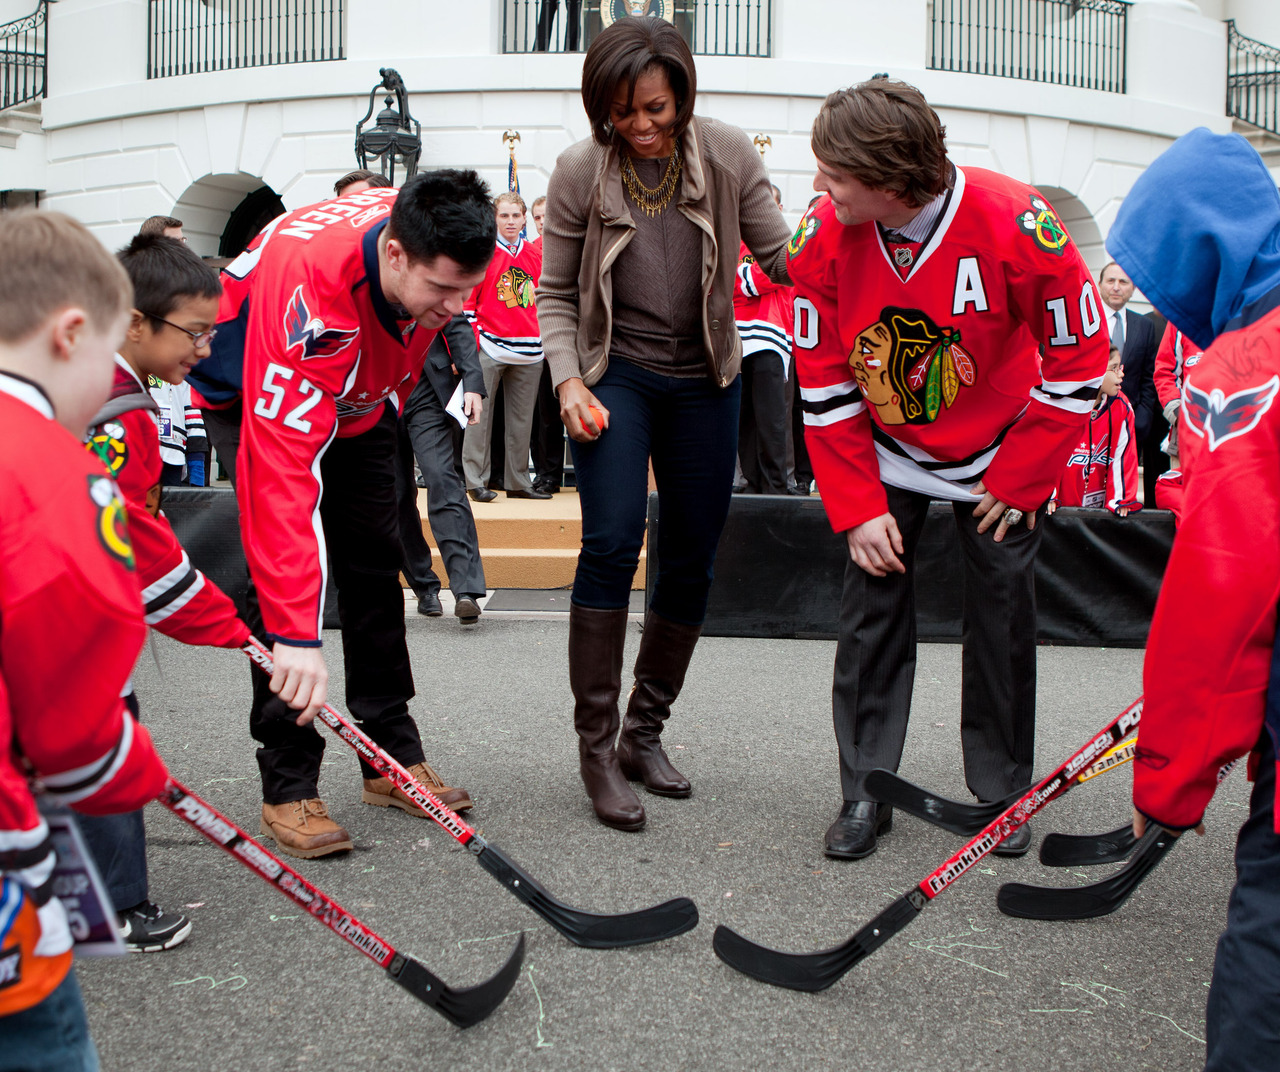
\includegraphics[height=4.7cm,width=\linewidth,keepaspectratio]{michelle_obama.jpg}\\[0.5em] Youth sports\end{column}
    \begin{column}{0.48\textwidth}\centering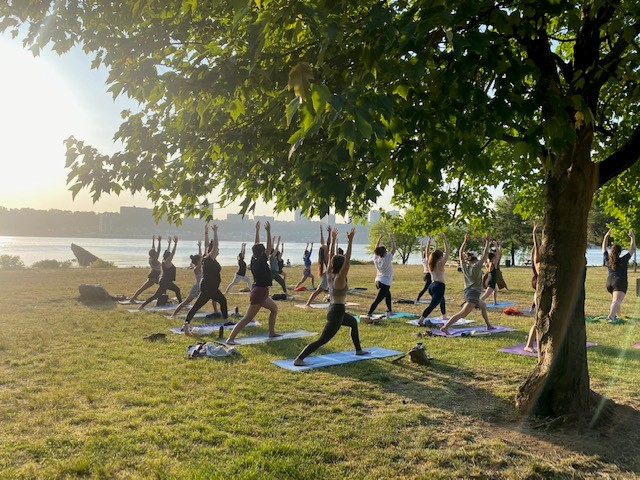
\includegraphics[height=4.7cm,width=\linewidth,keepaspectratio]{riverside_park_yoga.jpg}\\[0.5em] Exercise classes for old people\end{column}
  \end{columns}
\end{frame}
\begin{frame}{How can we promote this? \mdseries Smoking: anti-smoking ads}
  \centering
  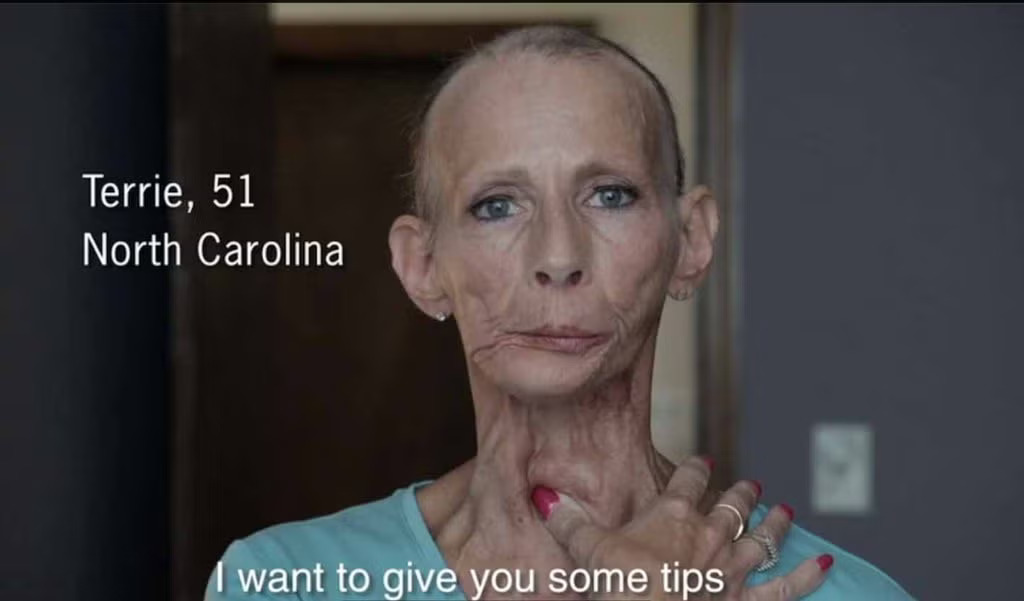
\includegraphics[height=5.9cm,width=\textwidth,keepaspectratio]{terrie.jpg}
  \source{Source: CDC, \emph{Tips From Former Smokers}.}
\end{frame}
\begin{frame}{How can we promote this? \mdseries Sleep}
  \begin{itemize}\setlength{\itemsep}{0.9em}
    \item There isn't really anything yet
    \item Important to have a \alert{regular} sleep schedule
  \end{itemize}
\end{frame}
\begin{frame}{Our Health Campaigns}
  \begin{columns}[c]
    \begin{column}{0.48\textwidth}\centering
\includegraphics[width=\linewidth]{tired_guy.jpg}\end{column}
    \begin{column}{0.48\textwidth}
      {\Large\bfseries\color{navy}Steven, 33\par}\vspace{0.6em}
      \begin{itemize}\setlength{\itemsep}{0.6em}
        \item Works 70 hours per week at a high-end law firm
        \item On average, sleeps 4 hours a night on weekdays, and 12 on weekends
        \item Family history of Alzheimer's
      \end{itemize}
    \end{column}
  \end{columns}
\end{frame}
\begin{frame}{Our Health Campaigns}
  \begin{columns}[c]
    \begin{column}{0.48\textwidth}\centering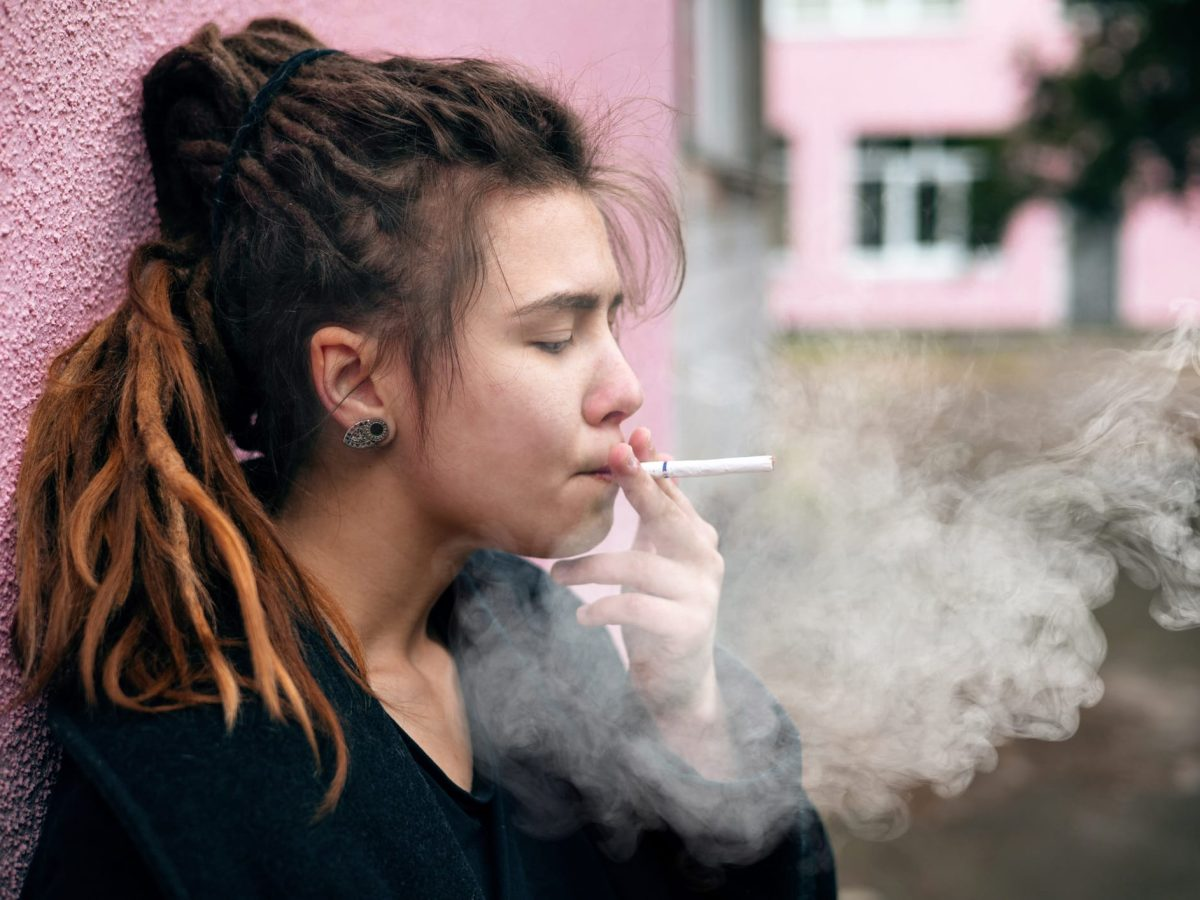
\includegraphics[width=\linewidth]{marie.jpg}\end{column}
    \begin{column}{0.48\textwidth}
      {\Large\bfseries\color{navy}Marie, 26\par}\vspace{0.6em}
      \begin{itemize}\setlength{\itemsep}{0.6em}
        \item Works at the ticket booth at a movie theater
        \item Started smoking at age 15 because it was cool
        \item Now smokes $\sim$10 cigarettes per day; says she needs to because of the stress
      \end{itemize}
    \end{column}
  \end{columns}
\end{frame}
\begin{frame}{Our Health Campaigns}
  \begin{columns}[c]
    \begin{column}{0.48\textwidth}\centering
\includegraphics[width=\linewidth]{gerald.jpg}\end{column}
    \begin{column}{0.48\textwidth}
      {\Large\bfseries\color{navy}Gerald, 45\par}\vspace{0.6em}
      \begin{itemize}\setlength{\itemsep}{0.6em}
        \item Semi-retired
        \item Lost 35 lbs last year from Ozempic
        \item Doesn't exercise because he says it's boring; injured his back last year
      \end{itemize}
    \end{column}
  \end{columns}
\end{frame}
\begin{frame}{Our Health Campaigns}
  \begin{columns}[T]
    \begin{column}{0.32\textwidth}\centering
\includegraphics[height=2.0cm,width=\linewidth,keepaspectratio]{tired_guy.jpg}\\[0.2em]
      {\large\bfseries\color{navy}Steven, 33\par}\vspace{0.1em}
      \footnotesize\begin{itemize}\setlength{\itemsep}{0.1em}\raggedright
        \item Works 70 hours per week at a high-end law firm
        \item On average, sleeps 4 hours a night on weekdays, and 12 on weekends
        \item Family history of Alzheimer's
      \end{itemize}
    \end{column}
    \begin{column}{0.32\textwidth}\centering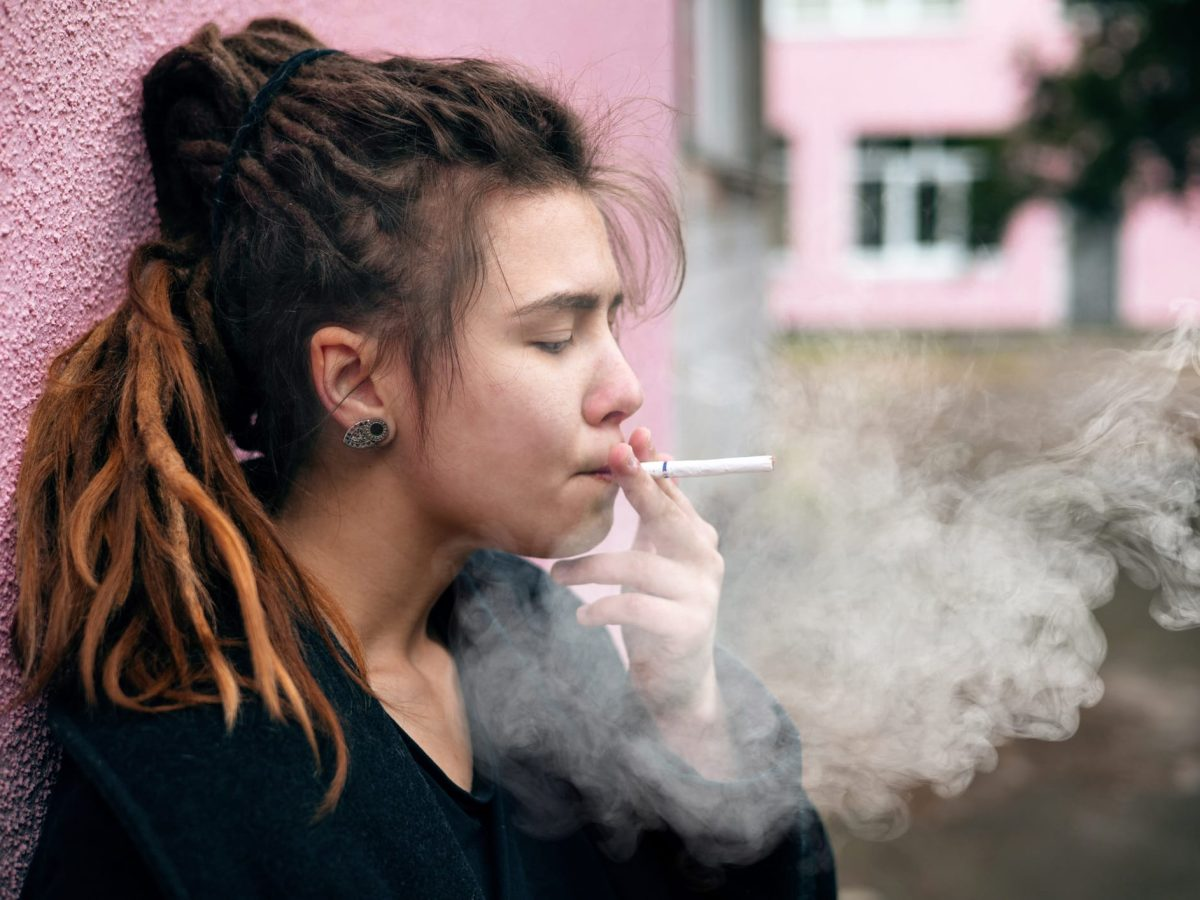
\includegraphics[height=2.0cm,width=\linewidth,keepaspectratio]{marie.jpg}\\[0.2em]
      {\large\bfseries\color{navy}Marie, 26\par}\vspace{0.1em}
      \footnotesize\begin{itemize}\setlength{\itemsep}{0.1em}\raggedright
        \item Works at the ticket booth at a movie theater
        \item Started smoking at age 15 because it was cool
        \item Now smokes $\sim$10 cigarettes per day; says she needs to because of the stress
      \end{itemize}
    \end{column}
    \begin{column}{0.32\textwidth}\centering
\includegraphics[height=2.0cm,width=\linewidth,keepaspectratio]{gerald.jpg}\\[0.2em]
      {\large\bfseries\color{navy}Gerald, 45\par}\vspace{0.1em}
      \footnotesize\begin{itemize}\setlength{\itemsep}{0.1em}\raggedright
        \item Semi-retired
        \item Lost 35 lbs last year from Ozempic
        \item Doesn't exercise because he says it's boring; injured his back last year
      \end{itemize}
    \end{column}
  \end{columns}
\end{frame}

\end{document}
